\documentclass[aspectratio=169,10pt]{beamer}
\usetheme{metropolis}
\usepackage{tikz}
\usetikzlibrary{calc,arrows.meta,shapes.geometric}

% ============================================================
% PRESENTATION META INFORMATION
% ============================================================
\title{Engineering Curves: Construction of Cycloid}
\subtitle{Animated Rolling Circle Method with Tangent \& Normal}
\author{Gajavada Sanjeevkumar}
\date{}

% ============================================================
% METROPOLIS NUMBERING
% ============================================================
\metroset{numbering=none}

% ============================================================
% CUSTOM FOOTER & STEP NUMBERING MACRO
% ============================================================
\newcommand{\stepnum}{0}

\setbeamercolor{custom footer}{fg=white,bg=black!80}

\setbeamertemplate{footline}{%
\leavevmode%
\hbox{%
\begin{beamercolorbox}[wd=\paperwidth,ht=3.2ex,dp=1.4ex,leftskip=1cm,rightskip=1cm]{custom footer}%
\tiny
\insertauthor
\quad|\quad
\inserttitle
\hfill
\ifnum\value{framenumber}=1
\textit{Introduction}%
\else
\ifnum\value{framenumber}=2
\textit{Problem Statement}%
\else
Step \stepnum
\fi
\fi
\end{beamercolorbox}%
}%
}

\setbeamertemplate{navigation symbols}{}

% ============================================================
% CUSTOM TIKZ STYLES & DEFINITIONS
% ============================================================
\tikzset{
  axis line/.style={thin,dash pattern=on 6pt off 2pt on 1.5pt off 2pt,black!75},
  directrix line/.style={ultra thick,magenta!90!black},
  construction line/.style={thin,blue!60!black},
  projection line/.style={thin,black!45},
  rolling circle/.style={thick,cyan!70!black},
  arc line/.style={thin,dashed,red!85!black},
  main curve/.style={ultra thick,magenta!90!black},
  tangent line/.style={thick,green!50!black},
  normal line/.style={thick,orange!80!black},
  point line/.style={thin,dashed,red!75!black},
  dimension line/.style={thin,<->,black!65},
  dimension extension/.style={thin,solid,black!60},
  >=Stealth,
}

\newcommand{\drawLegendCard}[1]{
\node[draw=gray!50,fill=white,rounded corners=4pt,inner sep=4pt,anchor=north east] at (20.9,8.65) {
\scriptsize
\begin{tabular}{l@{\,$\rightarrow$\,}l}
#1
\end{tabular}
};
}

\begin{document}

\begin{frame}[plain]
\titlepage
\end{frame}

\begin{frame}{Problem Statement}
\vfill
\begin{block}{Question}
Draw a \textbf{cycloid} generated by a circle of diameter $D=50\text{ mm}$ rolling along a straight base line for \textbf{one complete revolution without slipping}.
Construct a \textbf{tangent} and a \textbf{normal} to the cycloid at a selected point $P$.
\end{block}
\begin{alertblock}{Given}
$D = 50\text{ mm} \implies R = 25\text{ mm},\qquad \pi D \approx 157\text{ mm}$
\end{alertblock}
\vfill
\end{frame}

% ============================================================
% STEP 1: INITIAL CONFIGURATION
% ============================================================
\renewcommand{\stepnum}{1}
\begin{frame}{Step 1: Draw Directing Line and Generating Circle}
\centering
\begin{tikzpicture}[scale=0.52]
\useasboundingbox (-4.5,-3.5) rectangle (22.5,8.0);
\drawLegendCard{\textbf{$C_0$} & Initial centre \\ \textbf{$AA'$} & Directing line \\ \textbf{$R$} & Radius = 25 mm}
\coordinate (C0) at (0,3.0);
\draw[directrix line] (0,0) node[below left,font=\small] {$A$} -- (18.85,0) node[below right,font=\small] {$A'$};
\draw[axis line] (0,3.0) -- (18.85,3.0) node[right,font=\small] {$C_{12}$};
\fill[red!80!black] (C0) circle (3.5pt) node[above right,font=\small] {$C_0$};
\draw[rolling circle] (C0) circle (3.0);
\draw[<->,thin,cyan!80!black] (0,3.0) -- (0,0) node[midway,right,font=\tiny] {$R=25\text{ mm}$};
\end{tikzpicture}
\end{frame}

% ============================================================
% STEP 2: DIVIDE CIRCLE INTO 12 PARTS
% ============================================================
\renewcommand{\stepnum}{2}
\begin{frame}{Step 2: Divide Generating Circle into 12 Equal Parts}
\centering
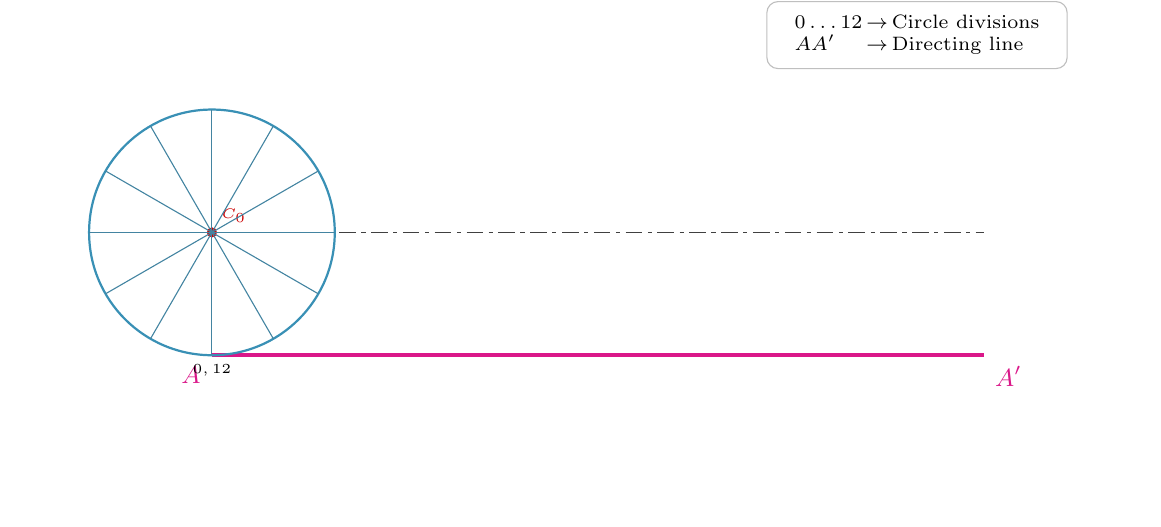
\begin{tikzpicture}[scale=0.52]
\useasboundingbox (-4.5,-3.5) rectangle (22.5,8.0);
\drawLegendCard{\textbf{$0\dots12$} & Circle divisions \\ \textbf{$AA'$} & Directing line}
\coordinate (C0) at (0,3.0);
\draw[directrix line] (0,0) node[below left,font=\small] {$A$} -- (18.85,0) node[below right,font=\small] {$A'$};
\draw[axis line] (0,3.0) -- (18.85,3.0);
\draw[rolling circle] (C0) circle (3.0);
\fill[red!80!black] (C0) circle (3.5pt) node[above right,font=\tiny] {$C_0$};
\draw[thin,cyan!60!black,solid] (C0) -- (0,0); \node[below,font=\tiny] at (0,0) {$0, 12$};
\foreach \i/\ang/\lbl in {1/300/1, 2/330/2, 3/0/3, 4/30/4, 5/60/5, 6/90/6, 7/120/7, 8/150/8, 9/180/9, 10/210/10, 11/240/11} {
  \draw[thin,cyan!60!black,solid] (C0) -- ++(\ang:3.0);
}
\end{tikzpicture}
\end{frame}

% ============================================================
% STEP 3: DIVIDE BASE LINE (PI*D)
% ============================================================
\renewcommand{\stepnum}{3}
\begin{frame}{Step 3: Divide Directing Line into 12 Equal Parts ($\pi D = 157$ mm)}
\centering
\begin{tikzpicture}[scale=0.52]
\useasboundingbox (-4.5,-3.5) rectangle (22.5,8.0);
\drawLegendCard{\textbf{$\pi D$} & Arc length ($157\text{ mm}$) \\ \textbf{1'--12'} & Base divisions}
\draw[directrix line] (0,0) node[below left,font=\small] {$A$} -- (18.85,0) node[below right,font=\small] {$A'$};
\draw[axis line] (0,3.0) -- (18.85,3.0);
\draw[dimension extension] (0,0) -- (0,-2.2);
\draw[dimension extension] (18.85,0) -- (18.85,-2.2);
\draw[<->,red!80!black,thin] (0,-1.8) -- (18.85,-1.8) node[midway,fill=white,font=\tiny] {$\pi D = 157\text{ mm}$};
\foreach \i in {1,2,...,12} {
  \fill[black] ({\i*1.5708}, 0) circle (1.8pt);
  \node[below,font=\tiny] at ({\i*1.5708}, 0) {\i'};
}
\end{tikzpicture}
\end{frame}

% ============================================================
% STEP 4: LOCATE CENTRES C1...C12
% ============================================================
\renewcommand{\stepnum}{4}
\foreach \n in {1,2,3,4,5,6,7,8,9,10,11,12} {
\begin{frame}{Step 4: Project Divisions to Locate Centres $C_1 \dots C_{12}$}
\centering
\begin{tikzpicture}[scale=0.52]
\useasboundingbox (-4.5,-3.5) rectangle (22.5,8.0);
\drawLegendCard{\textbf{$C_1\dots C_{12}$} & Path centres \\ \textbf{Axis Line} & Height = $R$}
\draw[directrix line] (0,0) node[below left,font=\small] {$A$} -- (18.85,0) node[below right,font=\small] {$A'$};
\draw[axis line] (0,3.0) -- (18.85,3.0);
\foreach \i in {1,2,...,12} {
  \fill[black] ({\i*1.5708}, 0) circle (1.8pt);
  \node[below,font=\tiny] at ({\i*1.5708}, 0) {\i'};
}
\pgfmathsetmaxmacro{\maxi}{\n}
\foreach \i in {1,...,\maxi} {
  \coordinate (C\i) at ({\i*1.5708}, 3.0);
  \draw[thin,black!40,solid] ({\i*1.5708}, 0) -- (C\i);
  \fill[red!80!black] (C\i) circle (2.5pt);
  \node[above=1pt,font=\tiny,red!80!black] at (C\i) {$C_\i$};
}
\end{tikzpicture}
\end{frame}
}

% ============================================================
% STEP 5: HORIZONTAL REFERENCE LINES
% ============================================================
\renewcommand{\stepnum}{5}
\begin{frame}{Step 5: Draw Horizontal Reference Lines from Circle Divisions}
\centering
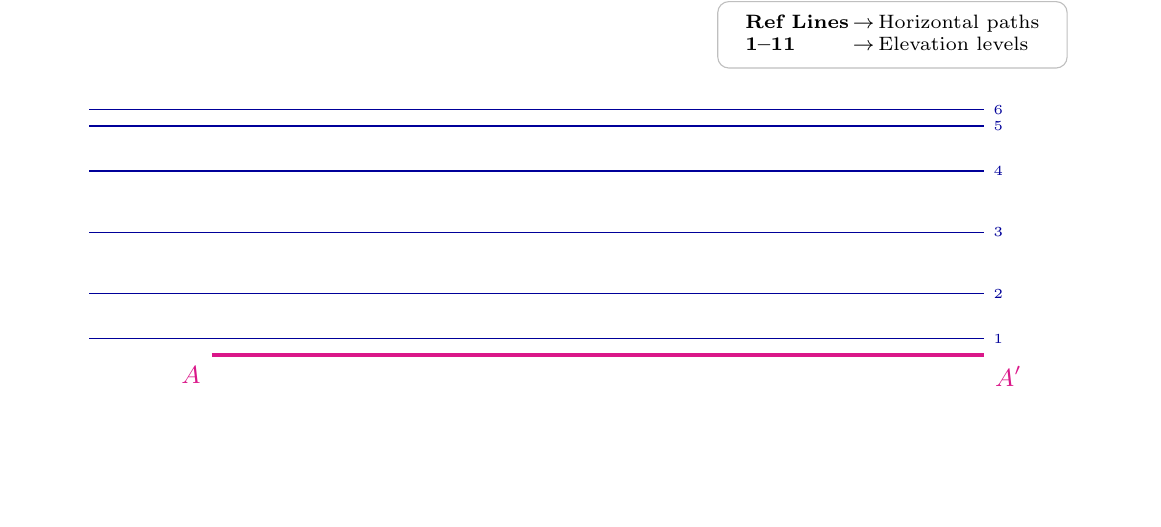
\begin{tikzpicture}[scale=0.52]
\useasboundingbox (-4.5,-3.5) rectangle (22.5,8.0);
\drawLegendCard{\textbf{Ref Lines} & Horizontal paths \\ \textbf{1--11} & Elevation levels}
\draw[directrix line] (0,0) node[below left,font=\small] {$A$} -- (18.85,0) node[below right,font=\small] {$A'$};
\draw[axis line] (0,3.0) -- (18.85,3.0);
\foreach \y/\lbl in {0.402/1, 1.500/2, 3.000/3, 4.500/4, 5.598/5, 6.000/6} {
  \draw[construction line] (-3.0, \y) -- (18.85, \y) node[right,font=\tiny] {\lbl};
}
\end{tikzpicture}
\end{frame}

% ============================================================
% STEP 6: LOCATE POINTS P1...P12 VIA ARCS
% ============================================================
\renewcommand{\stepnum}{6}
\foreach \n in {1,2,3,4,5,6,7,8,9,10,11,12} {
\begin{frame}{Step 6: Strike Cutting Arcs to Locate Point $P_\n$}
\centering
\begin{tikzpicture}[scale=0.52]
\useasboundingbox (-4.5,-3.5) rectangle (22.5,8.0);
\drawLegendCard{\textbf{$P_\n$} & Target point \\ \textbf{Radius} & $R = 25\text{ mm}$}
\draw[directrix line] (0,0) node[below left,font=\small] {$A$} -- (18.85,0) node[below right,font=\small] {$A'$};
\draw[axis line] (0,3.0) -- (18.85,3.0);
\foreach \i in {1,2,...,12} {
  \coordinate (C\i) at ({\i*1.5708}, 3.0);
  \fill[red!80!black] (C\i) circle (2.0pt);
}
% Draw up to current point n
\fill[blue!80!black] (0,0) circle (3pt) node[below left,font=\tiny] {$P_0$};
\ifnum\n>0 \draw[arc line] (1.5708,3.0) circle (3.0); \fill[blue!80!black] (1.5708,0.402) circle (3pt); \fi
\ifnum\n>1 \draw[arc line] (3.1416,3.0) circle (3.0); \fill[blue!80!black] (3.1416,1.500) circle (3pt); \fi
\ifnum\n>2 \draw[arc line] (4.7124,3.0) circle (3.0); \fill[blue!80!black] (4.7124,3.000) circle (3pt); \fi
\ifnum\n>3 \draw[arc line] (6.2832,3.0) circle (3.0); \fill[blue!80!black] (6.2832,4.500) circle (3pt); \fi
\ifnum\n>4 \draw[arc line] (7.8540,3.0) circle (3.0); \fill[blue!80!black] (7.8540,5.598) circle (3.pt); \fi
\ifnum\n>5 \draw[arc line] (9.4248,3.0) circle (3.0); \fill[blue!80!black] (9.4248,6.000) circle (3pt); \fi
\ifnum\n>6 \draw[arc line] (10.9956,3.0) circle (3.0); \fill[blue!80!black] (10.9956,5.598) circle (3pt); \fi
\ifnum\n>7 \draw[arc line] (12.5664,3.0) circle (3.0); \fill[blue!80!black] (12.5664,4.500) circle (3pt); \fi
\ifnum\n>8 \draw[arc line] (14.1372,3.0) circle (3.0); \fill[blue!80!black] (14.1372,3.000) circle (3pt); \fi
\ifnum\n>9 \draw[arc line] (15.7080,3.0) circle (3.0); \fill[blue!80!black] (15.7080,1.500) circle (3pt); \fi
\ifnum\n>10 \draw[arc line] (17.2788,3.0) circle (3.0); \fill[blue!80!black] (17.2788,0.402) circle (3pt); \fi
\ifnum\n>11 \draw[arc line] (18.8496,3.0) circle (3.0); \fill[blue!80!black] (18.85,0.000) circle (3pt); \fi
\end{tikzpicture}
\end{frame}
}

% ============================================================
% STEP 7: JOIN POINTS SMOOTHLY
% ============================================================
\renewcommand{\stepnum}{7}
\begin{frame}{Step 7: Smoothly Join Points to Form Cycloid Curve}
\centering
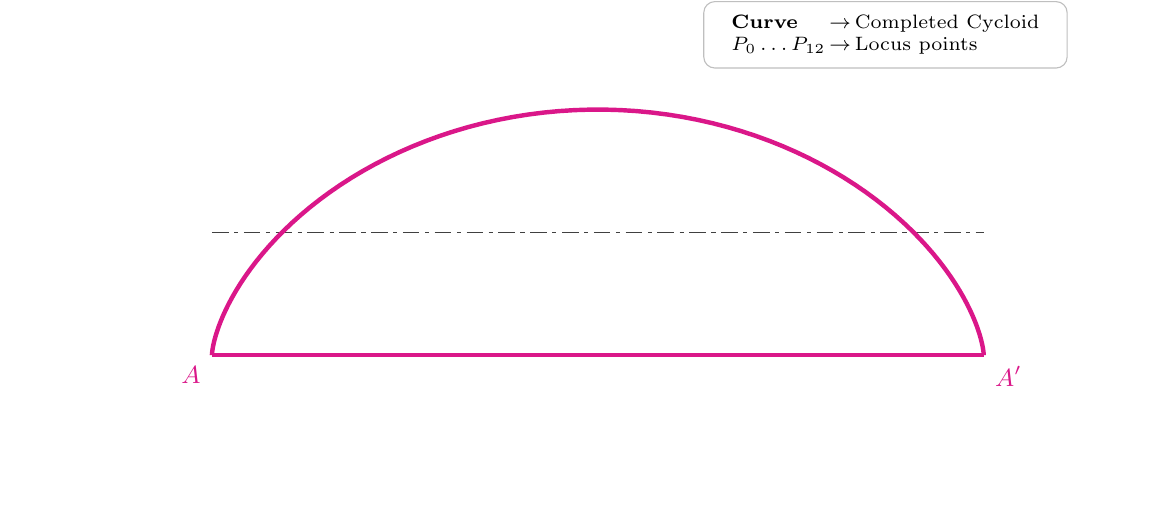
\begin{tikzpicture}[scale=0.52]
\useasboundingbox (-4.5,-3.5) rectangle (22.5,8.0);
\drawLegendCard{\textbf{Curve} & Completed Cycloid \\ \textbf{$P_0\dots P_{12}$} & Locus points}
\draw[directrix line] (0,0) node[below left,font=\small] {$A$} -- (18.85,0) node[below right,font=\small] {$A'$};
\draw[axis line] (0,3.0) -- (18.85,3.0);
\draw[main curve, samples=100, domain=0:6.28318] plot ({3*(\x - sin(\x r))}, {3*(1 - cos(\x r))});
\end{tikzpicture}
\end{frame}

% ============================================================
% STEP 8: SELECT POINT P & LOCATE CENTER Cp
% ============================================================
\renewcommand{\stepnum}{8}
\begin{frame}{Step 8: Select Point $P$ and Locate Corresponding Centre $C_p$}
\centering
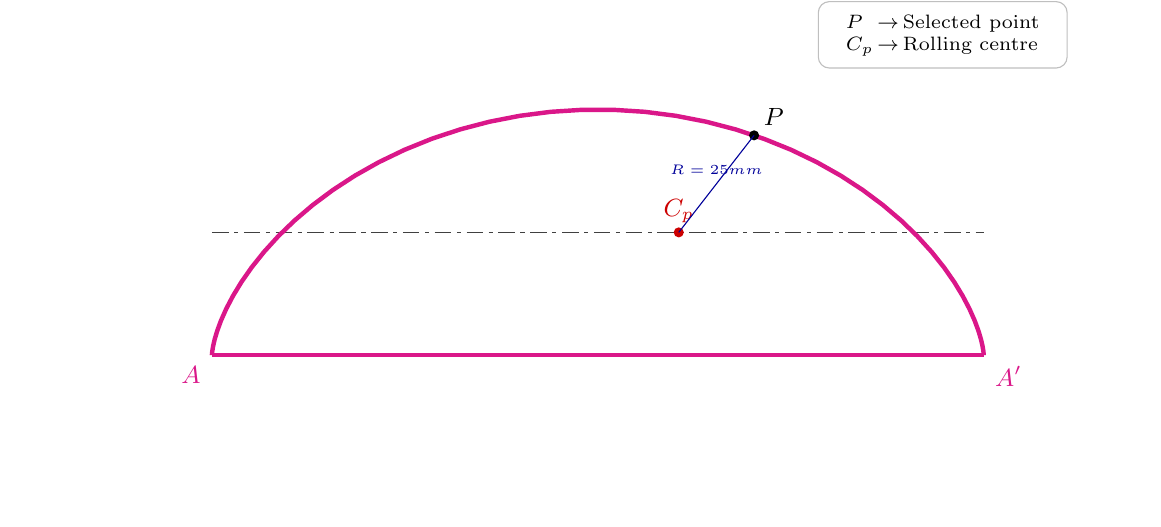
\begin{tikzpicture}[scale=0.52]
\useasboundingbox (-4.5,-3.5) rectangle (22.5,8.0);
\drawLegendCard{\textbf{$P$} & Selected point \\ \textbf{$C_p$} & Rolling centre}
\draw[directrix line] (0,0) node[below left,font=\small] {$A$} -- (18.85,0) node[below right,font=\small] {$A'$};
\draw[axis line] (0,3.0) -- (18.85,3.0);
\draw[main curve, samples=50, domain=0:6.28318] plot ({3*(\x - sin(\x r))}, {3*(1 - cos(\x r))});
\coordinate (P) at (13.24, 5.37);
\coordinate (Cp) at (11.40, 3.0);
\fill[black] (P) circle (3.5pt) node[above right] {\small $P$};
\fill[red!80!black] (Cp) circle (3.5pt) node[above] {\small $C_p$};
\draw[construction line] (P) -- (Cp) node[midway, above, font=\tiny] {$R=25\text{ mm}$};
\end{tikzpicture}
\end{frame}

% ============================================================
% STEP 9: NORMAL AND TANGENT CONSTRUCTION
% ============================================================
\renewcommand{\stepnum}{9}
\begin{frame}{Step 9: Construct Normal $N\text{-}N'$ and Tangent $T\text{-}T'$}
\centering
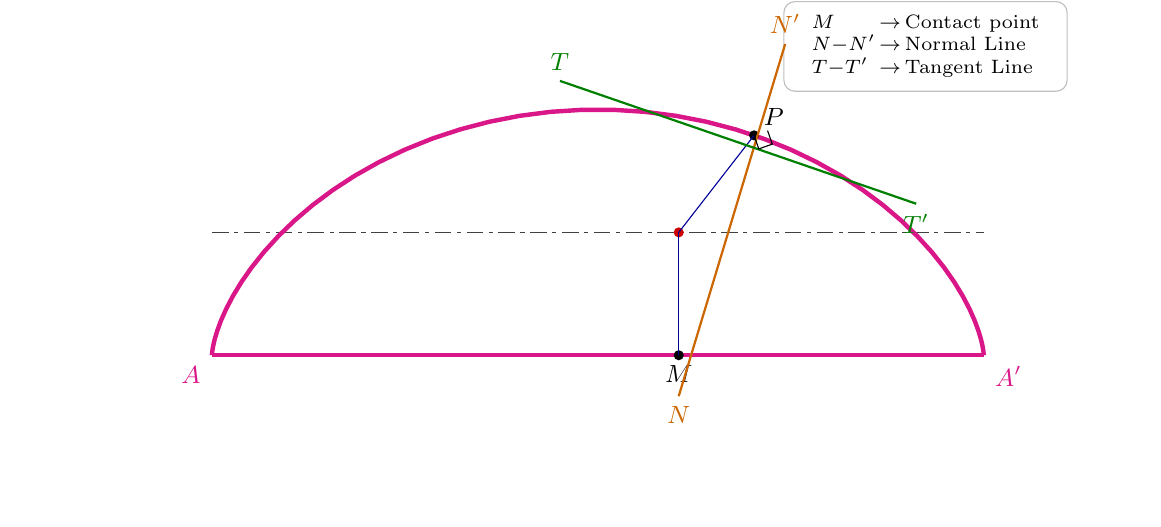
\begin{tikzpicture}[scale=0.52]
\useasboundingbox (-4.5,-3.5) rectangle (22.5,8.0);
\drawLegendCard{\textbf{$M$} & Contact point \\ \textbf{$N\text{-}N'$} & Normal Line \\ \textbf{$T\text{-}T'$} & Tangent Line}
\draw[directrix line] (0,0) node[below left,font=\small] {$A$} -- (18.85,0) node[below right,font=\small] {$A'$};
\draw[axis line] (0,3.0) -- (18.85,3.0);
\draw[main curve, samples=50, domain=0:6.28318] plot ({3*(\x - sin(\x r))}, {3*(1 - cos(\x r))});
\coordinate (P) at (13.24, 5.37);
\coordinate (Cp) at (11.40, 3.0);
\coordinate (M) at (11.40, 0.0);
\fill[black] (P) circle (3.5pt) node[above right] {\small $P$};
\fill[red!80!black] (Cp) circle (3.5pt);
\fill[black] (M) circle (3.5pt) node[below] {\small $M$};
\draw[construction line] (P) -- (Cp);
\draw[construction line, solid] (Cp) -- (M);
\draw[normal line] (11.40, -1.0) node[below] {\small $N$} -- (14.0, 7.6) node[above] {\small $N'$};
\draw[tangent line] (8.5, 6.7) node[above] {\small $T$} -- (17.2, 3.7) node[below] {\small $T'$};
\begin{scope}[shift={(13.24, 5.37)}, rotate=-70.7]
  \draw[thin, black] (0,0) -- (0.35,0) -- (0.35,0.35) -- (0,0.35);
\end{scope}
\end{tikzpicture}
\end{frame}

\end{document}
